\documentclass[conference]{IEEEtran}
\IEEEoverridecommandlockouts
% The preceding line is only needed to identify funding in the first footnote. If that is unneeded, please comment it out.
\usepackage{cite}
\usepackage{amsmath,amssymb,amsfonts}
\usepackage{algorithmic}
\usepackage{algorithm}
\usepackage{graphicx}
\usepackage{textcomp}
\usepackage{subfigure}


\def\BibTeX{{\rm B\kern-.05em{\sc i\kern-.025em b}\kern-.08em
    T\kern-.1667em\lower.7ex\hbox{E}\kern-.125emX}}
\begin{document}

\title{EEL 5840 Elements of Machine Intelligence\\ Project 2: Multilayer Perceptron - MNIST Dataset\\
%{\footnotesize \textsuperscript{*}}
}

\author{\IEEEauthorblockN{Hudanyun Sheng}
\IEEEauthorblockA{\textit{Industrial and Systems Engineering} \\
\textit{University of Florida}\\
Gainesville, United States \\
hdysheng@ufl.edu}


}

\maketitle

\begin{abstract}
In this paper, the famous MNIST dataset is examined using multilayer perception. Architecture of single hidden layer neural network is trained using training data, and tested with test data. The number of units in each layer is experimented with and discussed. The performance for the networks are reported on the test set with confusion matrices. Principal component analysis is used as dimensionality reduction approach, and the performances are compared with or without dimensionality reduction. Learning curves comparing training and validation cost function are shown, and the accuracies are compared. The performances with Stochastic Gradient Descent and SGD-momentum are compared. 
\end{abstract}

\begin{IEEEkeywords}
multilayer perceptron, stochastic gradient descent, learning curves, backpropagation, delta rule
\end{IEEEkeywords}

\section{Introduction}
The MNIST database (Modified National Institute of Standards and Technology database) is a large database of handwritten digits that is commonly used for training various image processing systems as well as training and testing in the field of machine learning. It was created by "re-mixing" the samples from MNIST's original datasets\cite{b1}. The MNIST database contains 60,000 training images and 10,000 testing images.

Neural networks, or properly referred to as an artificial neural network (ANN), can be defined as ``learning machines built from many different processing elements"\cite{b2}. An simple example of neural network with two hidden layers is shown in figure \ref{ANN}:
\begin{figure}[htbp]
\centerline{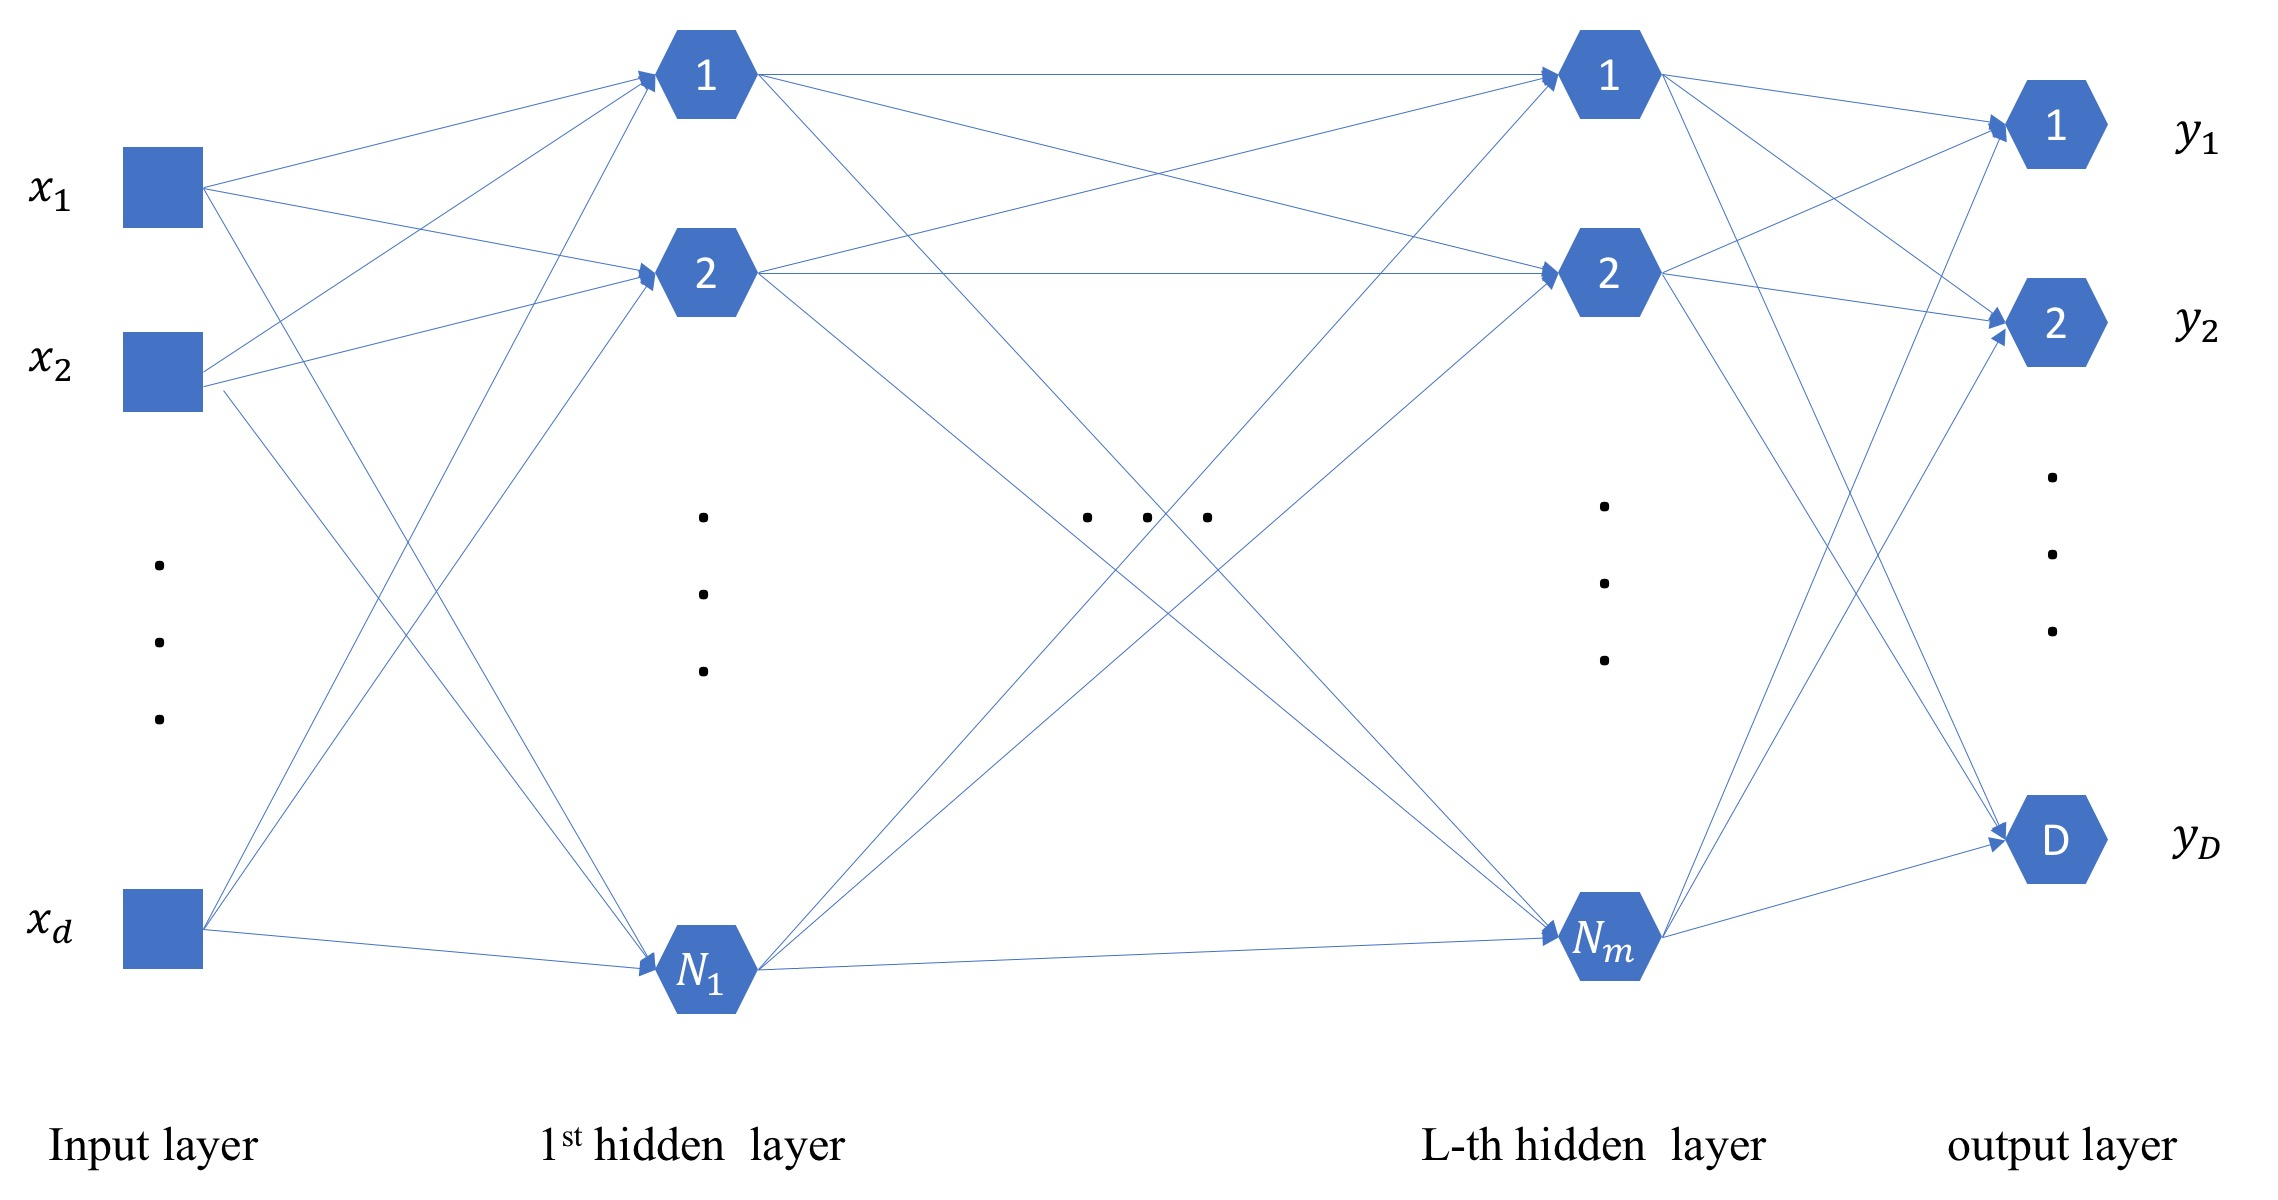
\includegraphics[width=3.4in]{annBlock.jpg}}
\caption{Multi-layer Perceptron with 2 Hidden Layers.}
\label{ANN}
\end{figure}

Although there are many different kinds of learning rules used by neural network, the one discussed and used in this paper is the delta rule. The delta rule is often used by the most common class of ANNs called ``backpropagational neural networks" (BPNNs). Backpropagation is an abbreviation for the backwards propagation of error.

The task fulfilled and discussed regarded in this paper is to train a multilayer perceptron on the MNIST data set with 50,000 training images and use last 10,000 images in the training dataset as validation set for cross-validation, then the model is tested on the test images. Single hidden layer neural networkis discussed in this paper. 

The rest of the paper is organized as follows. Section \uppercase\expandafter{\romannumeral2} describes the methodology being used in this paper. Section  \uppercase\expandafter{\romannumeral3} shows the results of the experiments. Section  \uppercase\expandafter{\romannumeral4} includes some discussion regarding this problem. And section \uppercase\expandafter{\romannumeral5} makes concluding remarks and discusses future lines of research.

\section{Methodology}
\subsection{Artificial neural network} An artificial neural network is a set of interconnected processing elements. A processing unit receives input from external sources, and by propagate over every unit in every layer, it is able to obtain a final output.
\paragraph {Single processing element}
If look at single processing element(SE, neuron), as shown in figure \ref{PE}, it takes the sum product of all the input values with weight vectors added bias as the input of the neuron, and after some type of activation function, the output of this neuron is obtained:
$$y_i = f(z_i)$$
where $z_i = \sum_{i=1}^n w_{ik}x_{ik}+b_{i}$. And in our case the activation function as selected to be ReLU function. The rectified linear unit(ReLU) function is defined as:
$$f(x) = x^{+} = max(0,x)$$
\begin{figure}[h!]
\centerline{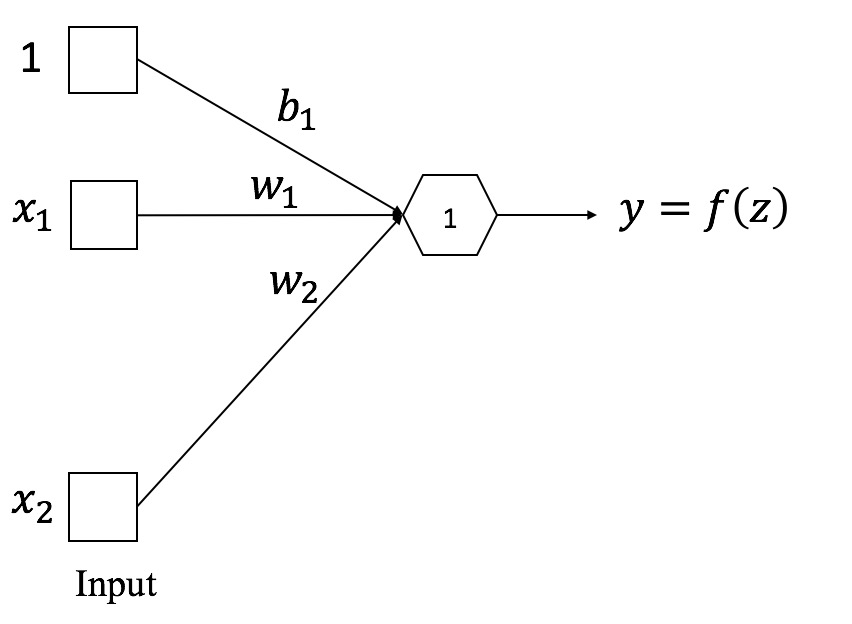
\includegraphics[width=3.4in]{sPE.jpg}}
\caption{Single processing element of an artificial neural network.}
\label{PE}
\end{figure}
\paragraph {Multilayer Perceptrons}
%Taken one hidden layer neural network as example, as shown in figure \ref{ANN1}, 
%\begin{figure}[htbp]
%\centerline{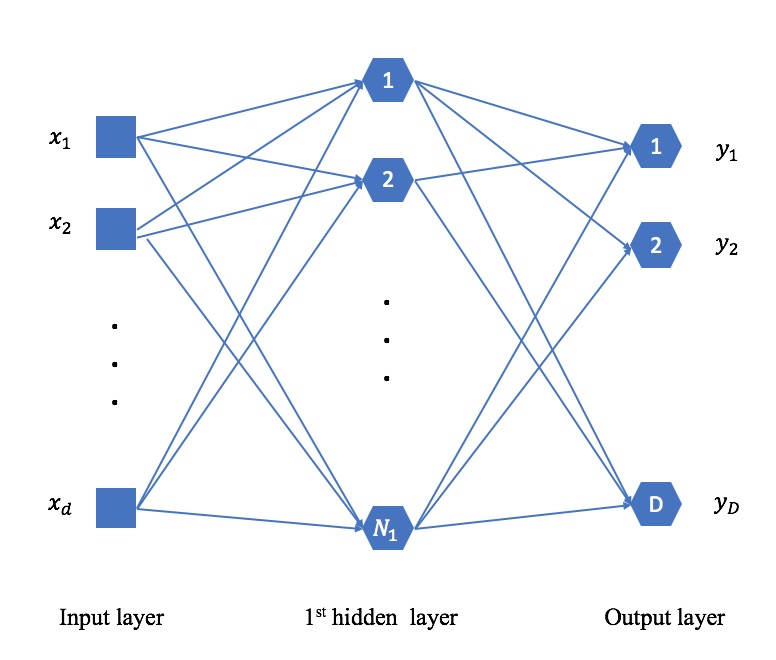
\includegraphics[width=3.4in]{block1hidden.jpg}}
%\caption{Artificial neural network with 1 Hidden Layer.}
%\label{ANN1}
%\end{figure}the dimensionality of the input layer depend on the dimensionality of the input train data, the number of units in 1-st hidden layer (and potentially 2-nd hidden layer) is the hyper-parameter to be decided, the output dimension is actually set to be ten, since there are only 10 different outputs, i.e. the number from 0 to 9. \\
As shown in figure \ref{ANN}, suppose the multilayer perceptron has L hidden layers, the $l^{th}$ hidden layer consists of $N_{l}$ hidden units. The output value of i-th unit in l-th hidden layer is 
$$y_{j}^l = f(\sum_{n=1}^{N_l}w_{ij}^{(l)}y_i^{l-1}+b_i^{l})$$
where, $w_{ij}$ represents for the weights, and $b_{i}$ represents for the biases regarding i-th unit of l-th layer. 
\subsection {Backpropagation} The cost function used here is the mean-of-squared error function, which is defined to be 
$$E(w)= \sum_{n=1}^N E_n(w) = \displaystyle\frac{1}{2N}\sum_{n=1}^N\sum_{i=1}^N(y_i(x_n,w)-t_{ni})^2$$
where $t_{ni}$ represents for the i-th entry of the n-th target value. The update of weights as well as biases are determined by a parameter optimization algorithm to minimize the error\cite{b6}, i.e. 
$$\nabla E(w) = 0$$
where $\nabla E(w) = 0$ represent for the gradient of the cost function. And the weights (as well as biases) are updated using stochastic gradient descent :
$$w(t+1) = w(t)+\eta \Delta w(t)$$
If focusing on an neural in the output layer, it is easy to get from train rule that:
$$\frac{\partial{E}}{\partial{w_{ij}}} = \frac{\partial{E}}{\partial{y_p}}\frac{\partial{y_p}}{\partial{net_p}} \frac{\partial{net_p}}{\partial{w_{ij}}} =-(d_p-y_p)f'(net_p)x_{ip}$$
where $(d_p-y_p) = \epsilon$ is defined as the error term of a single unit.\\
So that the update equation for weights can be written as:
$$w_{ij}(n+1) = w_{ij}(n)+\eta \epsilon_p(n)x_{ip}(n)f'(net_p)$$
similarly, the update equation for biases can be written as:
$$b_i(n+1) = b_i(n)+\eta \epsilon_p(n)f'(net_p)$$
This is the famous ``Delta Rule".\\
$\delta_{ip} = -(d_p-y_p)f'(net_p)$ is defined as the ``local error". Only the output layer has ``desired value", and thus the error term can be defined; for the hidden layers, the error term is defined as $\delta_i = \sum_j w_{ij}\delta_j$, taking the summation over all weight coming from neuron i times the local error of each of them.

And the rule of backpropagation can be derived like this: there are 2 signals in a neural network - forward and backward. The forward signal is the function signal while the backward signal represent for the error signal. Thus the training procedure of a neural network should also contain two parts: forward pass and backward pass. In the forward pass, the input vector go through all the neurons until the outputs on the output layer are gained. And then, starting from comparing the output with the desired output values, using delta rule, with back propagation, the network learns the pattern from the training data. 
\paragraph{Training Approaches}
To train an artificial neural network model, we first define a cost function, in this case the sum of squared error function is used as stated before; then we pick an activation function, in this paper we only ReLU is used and discussed for faster convergence; then a step size $\eta$ is chosen; the weights and biases are initialized randomly, with online training method, every iteration an input value $x_n$ is chosen randomly and propagate it through the network, the weights and biases are updated based on the error $E_n(w)$. When all training samples complete this procedure, one epoch of training finishes. The whole procedure should repeat until converge. An online learning procedure is used for the whole procedure. The pseudocode is shown below:
\begin{algorithm}
    \caption{Artificial Neural Network Training Algorithm}
    \begin{algorithmic}[1]
        \renewcommand{\algorithmicrequire}{\textbf{Input:}}
        \renewcommand{\algorithmicensure}{\textbf{Output:}}
        \REQUIRE Training data, step size $\eta$
        \ENSURE  Classification labels
        \\ \textit{Define number of hidden layers $L$, number of hidden units for every layer $N_l$, activation function $f(x)$}
        \FOR {epoch= 1:max epoch}
        \STATE shuffle input samples
        \FOR {iteration = num of training samples}
        \STATE Initialize weights and biases randomly
        \STATE    Forward pass with sample n: \\
        $y_j^l = f(\sum_{n=1}^{N_l}w_{ij}^{l-1}y_i^{l-1}+b_i^l)$
        \STATE  Backward pass with sample n
        \STATE     Update weights $w_{ij}$ and biases $b_i$
        \ENDFOR
        \ENDFOR
    \end{algorithmic}
\end{algorithm}

\paragraph{Update with momentum}
As is known to all, for any learning procedure regarding gradient descent, the choice of learning rate is really crucial. If the learning rate $\eta$ is too small, the learning procedure would be slow and take a long time to converge, if the learning rate $\eta$ large, there would be large changes in the synaptic weights, and may cause osillation. One way to trying to increase rate of learning while avoiding instability is including a momentum term to the gradient of the cost function, i.e.
$$\Delta w(n) = \eta\displaystyle\frac{\partial E}{\partial w(n)} + \alpha \Delta w_{(n-1)}$$
where $\alpha$ is a hyper-parameter to be picked, and $0\leq |\alpha| <1$. Based on the inclusion of the momentum term, the update equation becomes 
$$w_{ij}(n+1) = w_{ij}(n) + \eta \epsilon_p(n)x_{ip}f'(net_p)+\alpha \eta  \Delta w_{ij}{(n)}$$
$$b_i(n+1) = b_i(n) + \eta \epsilon_p(n)f'(net_p)+\alpha \eta  \Delta b_i{(n)}$$
How this method works can be interpreted like this: the change in weight (bias) becomes dependent on the previous change in weight (bias), where the larger the previous change will encourage the change in the current one. So the inclusion of momentum accelerate descent in steady downhill directions, and also has a stabilizing effect in directions that oscillate in sign. The training procedure with inclusion of momentum would be pretty much the same, only the change in pseudocode would be the update equation for weights and biases as mentioned before.

\paragraph{Regularization with dropout} 
Apart from using a validation set for early stopping or L1 or L2 regularization to prevent the network from overfitting, as introduced by Srivastava et al., another effective and simple way to prevent network from overfitting is dropout\cite{b4}. As shown in figure \ref{Dropout} the comparison of the basic operations of a standard and dropout network. As discussed before, a standard network can be described as:
$$y_i^{l+1} = f(w_i^{l+1}y^l+b_i^{l+1})$$
With dropout, the forward pass of the network becomes:
$$r_j^{l+1}\sim Bernoulli(p)$$
$$\tilde{y}^{l} = r^{l} * y^{l}$$
$$y_i^{l+1} = f(w_i^{l+1}\tilde{y}^{l}+b_i^{l+1})$$
Here $*$ represent for an element-wise product. For any layer, $r^l$ is a vector of independent Bernoulli random variables with each has set probability $p$ of being 1. The $l$-th layer of the network is thus thinned by this dropout procedure, and $\tilde{y}^{(l)}$ is then used as input to the next layer. This method works as sampling a sub-network from a larger network. It has to be mentioned here, when it comes to the test (predict) stage, scaling for layers with the dropout procedure with $p$ is necessary.
\begin{figure}[htbp]
\centerline{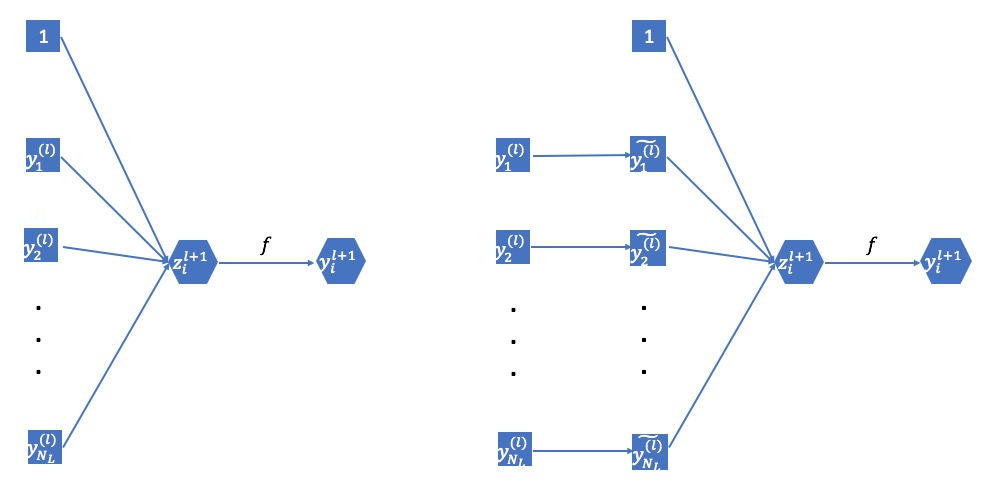
\includegraphics[width=3.6in]{dropout.jpg}}
\caption{Schematic diagram of network dropout. Left: standard network. Right: Dropout network}
\label{Dropout}
\end{figure}


\subsection{Principal component analysis} Inspired from the Curse of dimensionality, when in high dimensional spaces, much of the space is empty and the data lives at the surface. Thus, given the data set is of high dimensionality, i.e. dimension of 784, dimensionality reduction is necessary. Principal component analysis is used to reduce dimensionality. PCA is a very common and simplest approach to dimensionality reduction, which uses a linear transformation to minimize the redundancy of the resulting transformed data.
	
\section{Results}
\subsection{Dimensionality reduction} 

dimensionality reduction is necessary. The question encountered is how many dimensions to keep. Shown in figure \ref{PCA} is the plot of fraction of total variance retained with number of eigenvalues. This figure gives us a hint of approximately how many dimension to retain.
\begin{figure}[h!]
\centerline{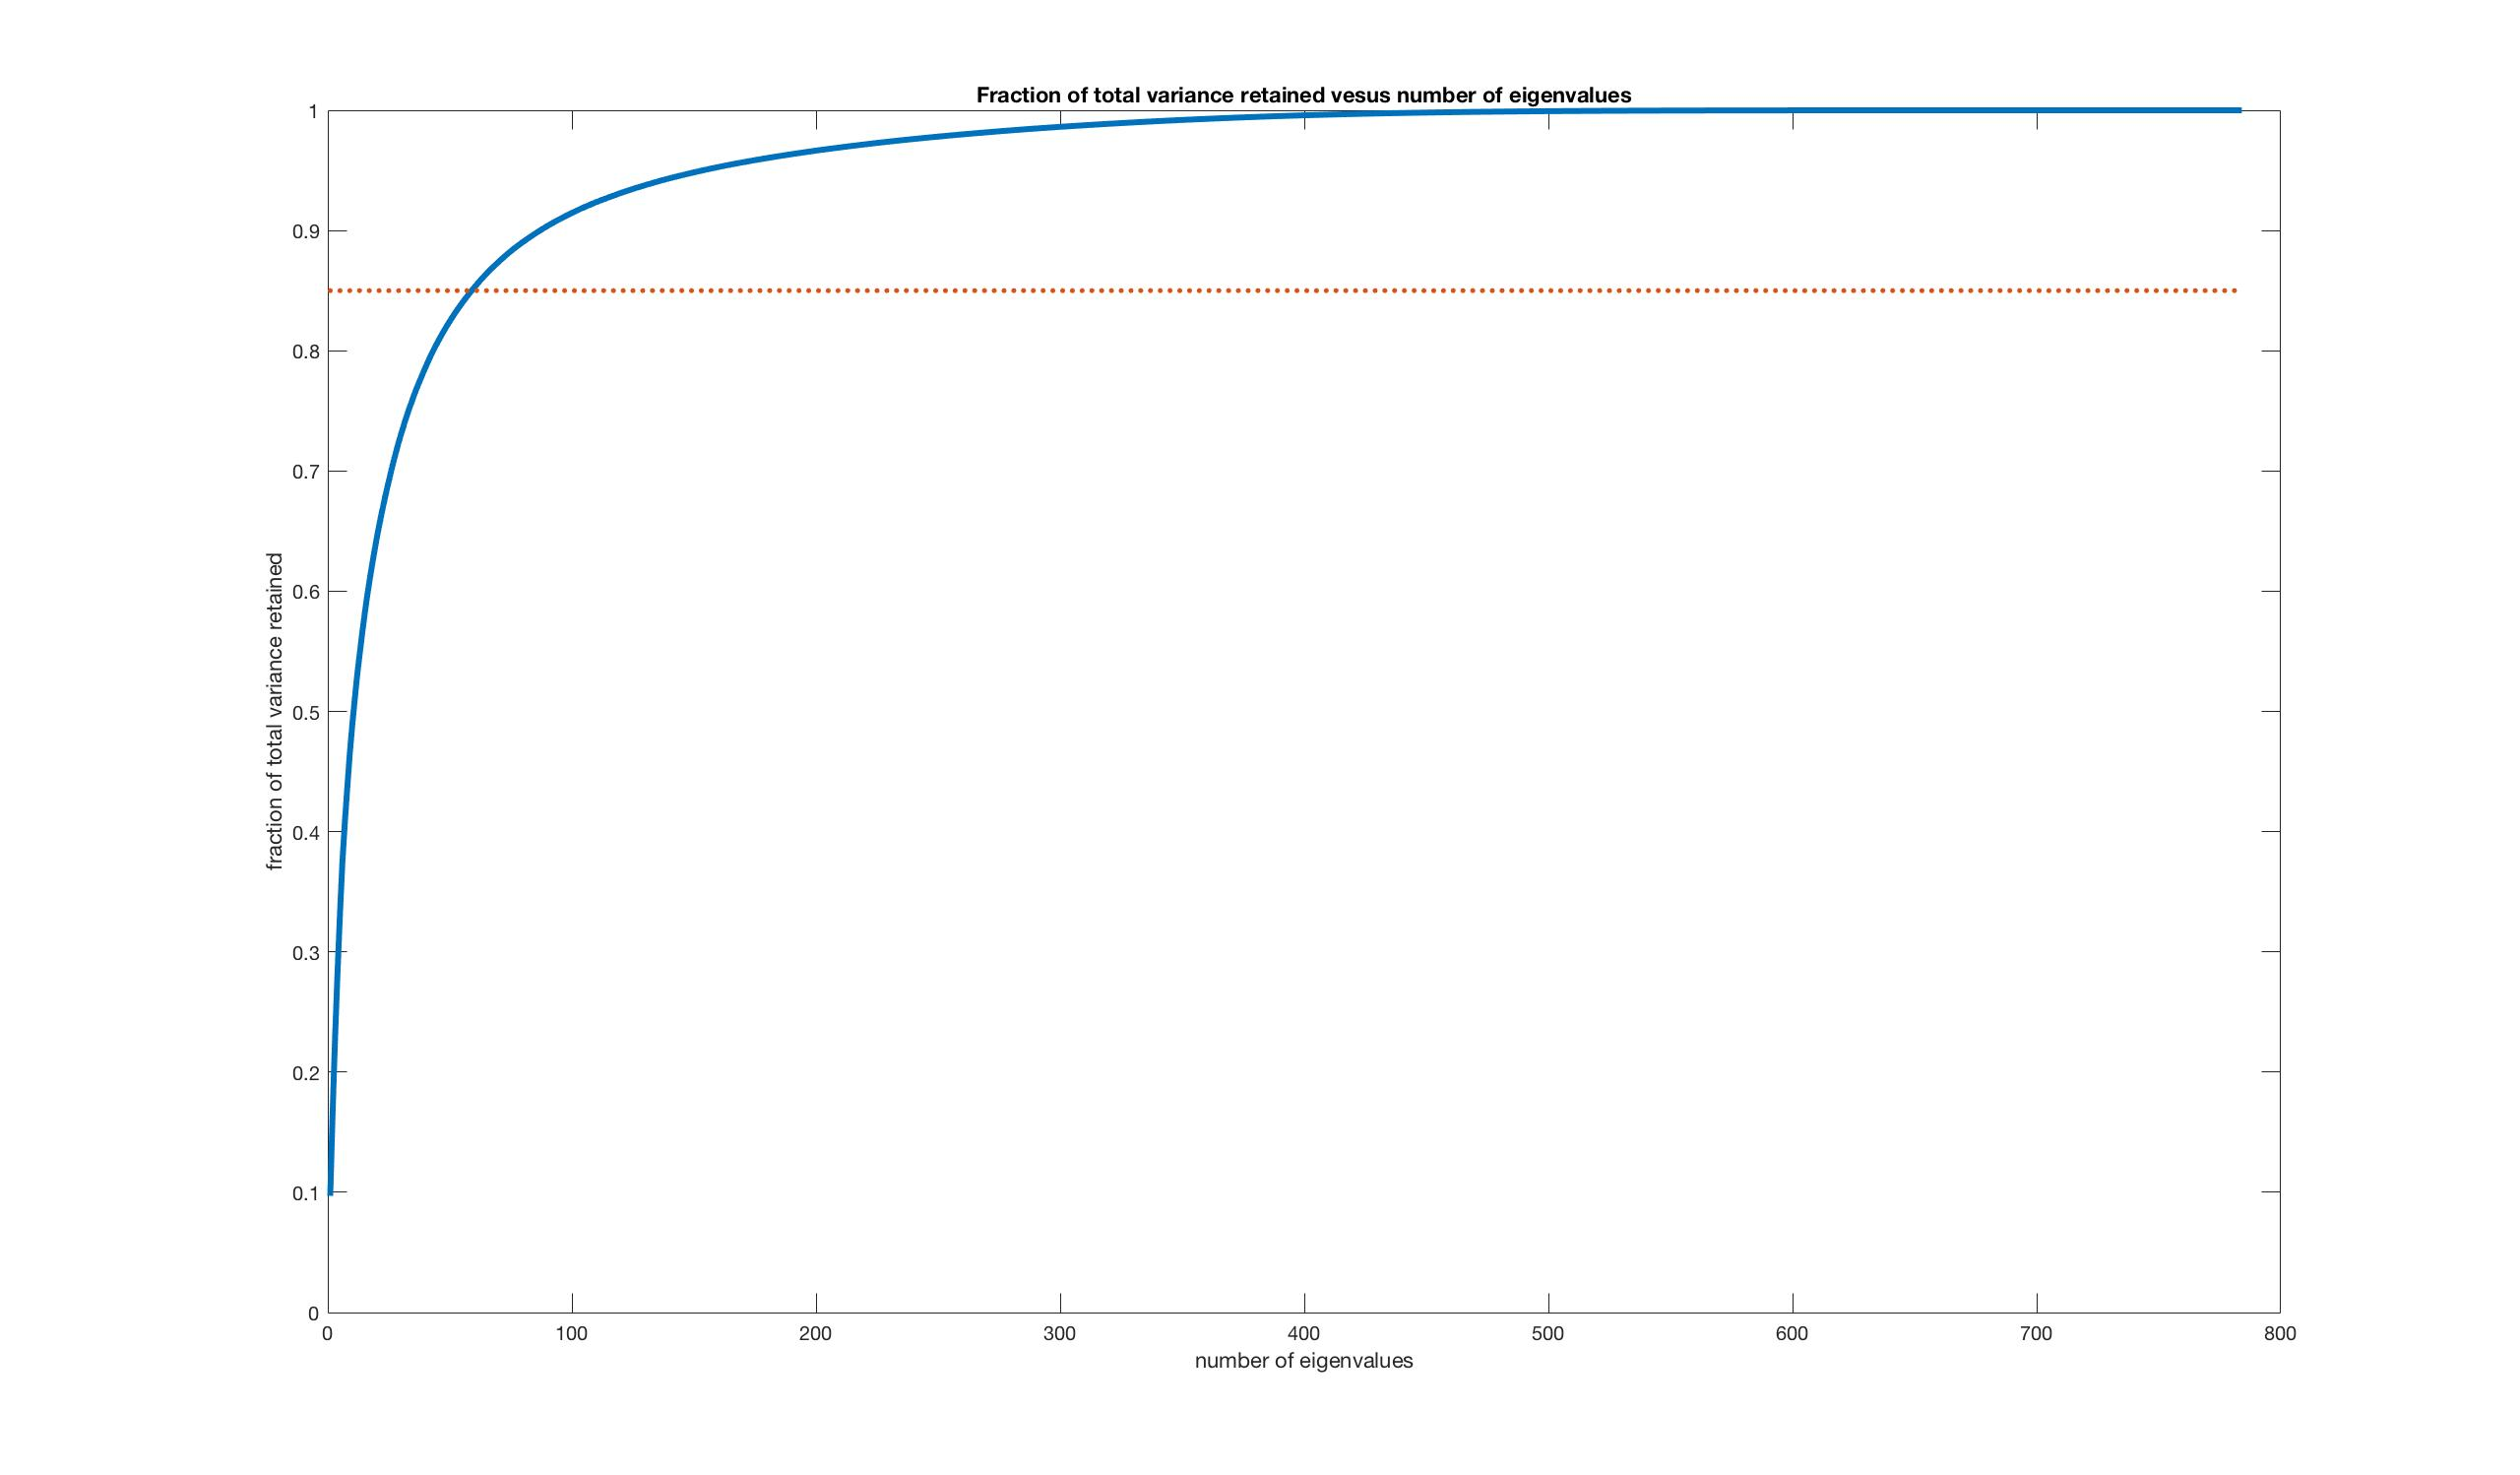
\includegraphics[width=3.4in]{PCA.jpg}}
\caption{Plot of fraction of total variance retained vs. number of eigenvalues}
\label{PCA}
\end{figure}

The dimension to retain differ from problem to problem. But generally speaking, if the dimensionality being kept can represent at least $85\%$ of the total variance, it should be enough. Though further experiments would be needed to compare the performance. Considering the time-accuracy trade-off, project the original data onto a subspace with dimension of 100 is able to retain $90\%$ of the total variance of the original data, would be a good starting point.

\subsection{One hidden layer neural network} Regarding to deciding number of hidden units when using single layer neural network, experiments with different models are done and results are compared. The number hidden units are chosen to be 50, 100, 200, 300, 400, 500, 600, 700, 800, 900, 1000, 1500, 2000. The step size is chosen to be $\eta = 0.01$, The iterations over entire training set is set to be 500 to promise convergence. Selected learning curves as well as the accuracy curves are shown below in figures \ref{1hidden100} to figure \ref{1hidden800}. And the plot of error bar is shown in \ref{errorBar}.

\begin{figure}[h!]
\centerline{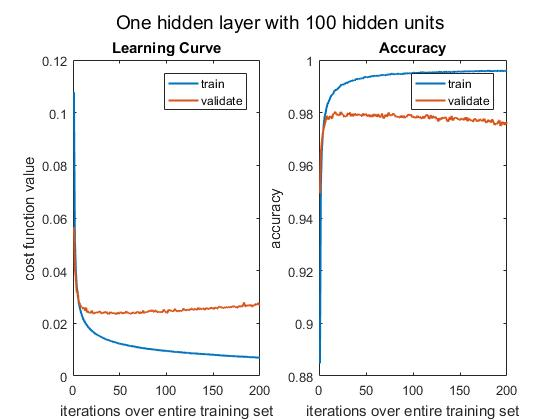
\includegraphics[width=3.5in]{LCAC100.jpg}}
\caption{Left: learning curve of train set as well as validation set with 100 hidden units. Right: accuracy curve of train set as well as validation set with 100 hidden units.}
\label{1hidden100}
\end{figure}

%\begin{figure}[htbp]
%\centerline{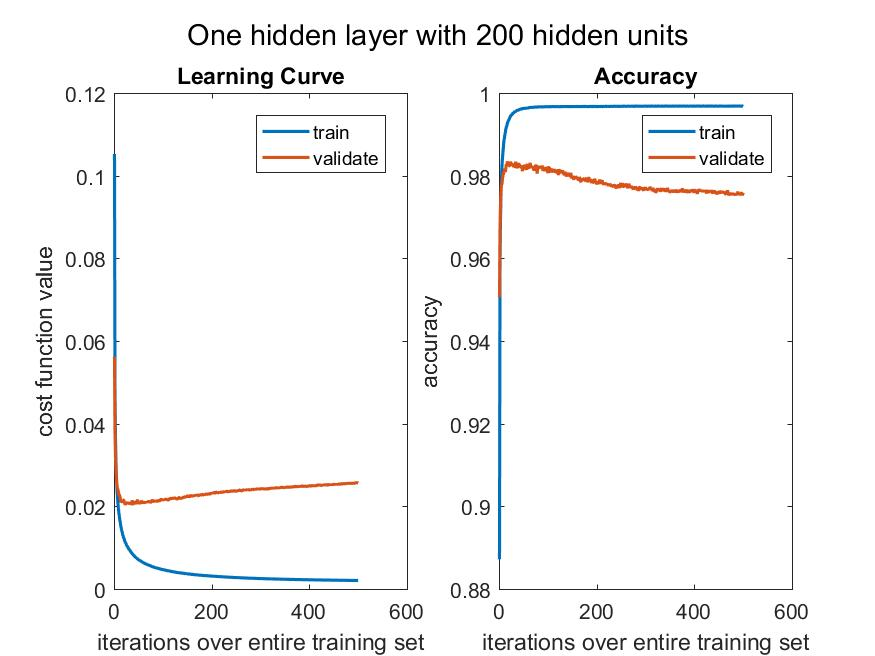
\includegraphics[width=3.5in]{LCAC200unitsPCA100eta.jpg}}
%\caption{Left: learning curve of train set as well as validation set with 200 hidden units. Right: accuracy curve of train set as well as validation set with 200 hidden units..}
%\label{1hidden200}
%\end{figure}

%\begin{figure}[htbp]
%\centerline{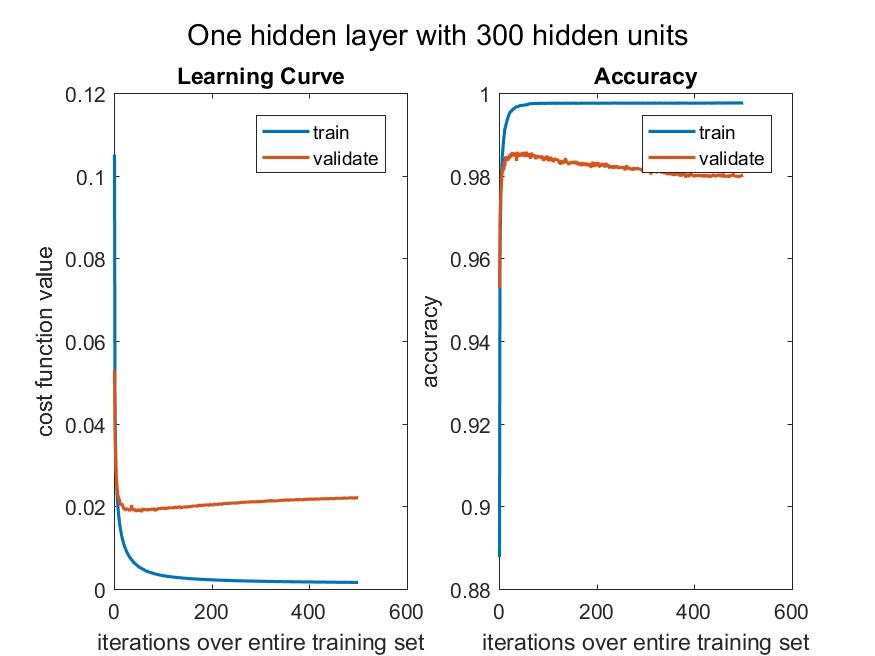
\includegraphics[width=3.5in]{LCAC300unitsPCA100eta.jpg}}
%\caption{Left: learning curve of train set as well as validation set with 300 hidden units. Right: accuracy curve of train set as well as validation set with 300 hidden units.}
%\label{1hidden300}
%\end{figure}

\begin{figure}[h!]
\centerline{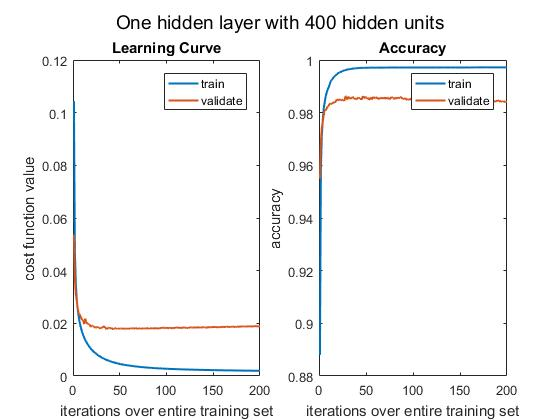
\includegraphics[width=3.5in]{LCAC400.jpg}}
\caption{Left: learning curve of train set as well as validation set with 400 hidden units. Right: accuracy curve of train set as well as validation set with 400 hidden units.}
\label{1hidden400}
\end{figure}

%\begin{figure}[htbp]
%\centerline{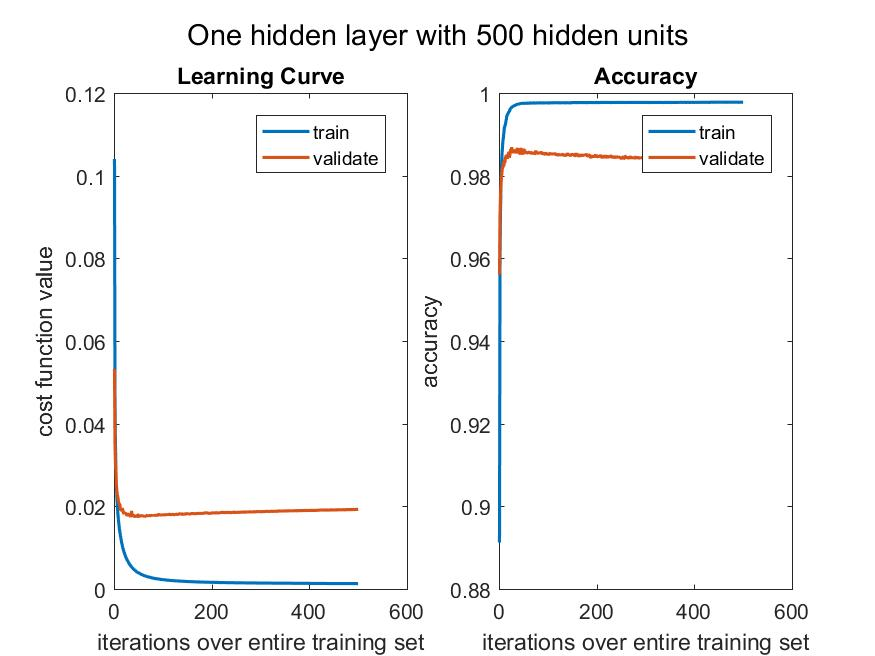
\includegraphics[width=3.5in]{LCAC500unitsPCA100eta.jpg}}
%\caption{Left: learning curve of train set as well as validation set with 500 hidden units. Right: accuracy curve of train set as well as validation set with 500 hidden units.}
%\label{1hidden500}
%\end{figure}

%\begin{figure}[htbp]
%\centerline{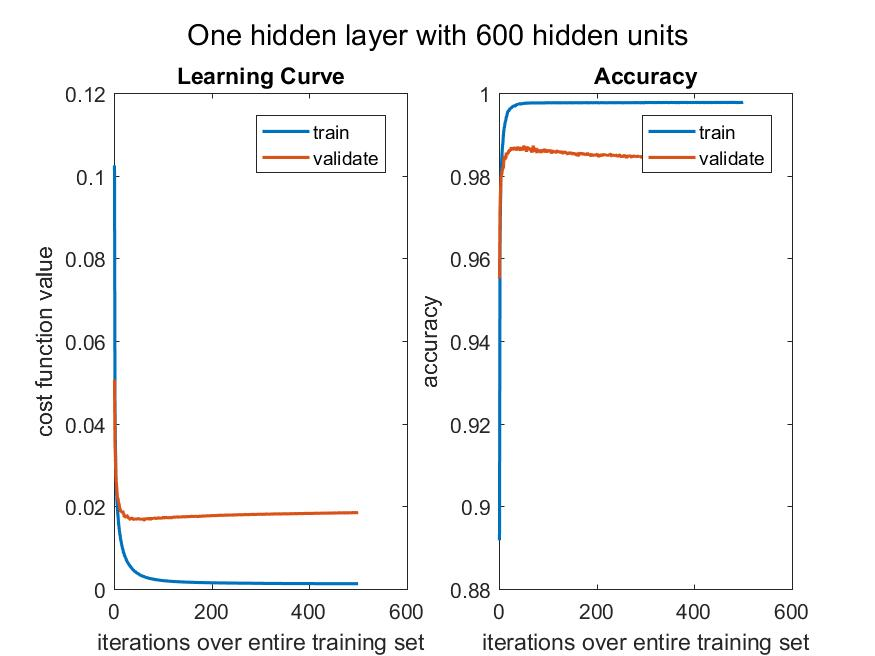
\includegraphics[width=3.5in]{LCAC600unitsPCA100eta.jpg}}
%\caption{Left: learning curve of train set as well as validation set with 600 hidden units. Right: accuracy curve of train set as well as validation set with 600 hidden units.}
%\label{1hidden600}
%\end{figure}

\begin{figure}[htbp]
\centerline{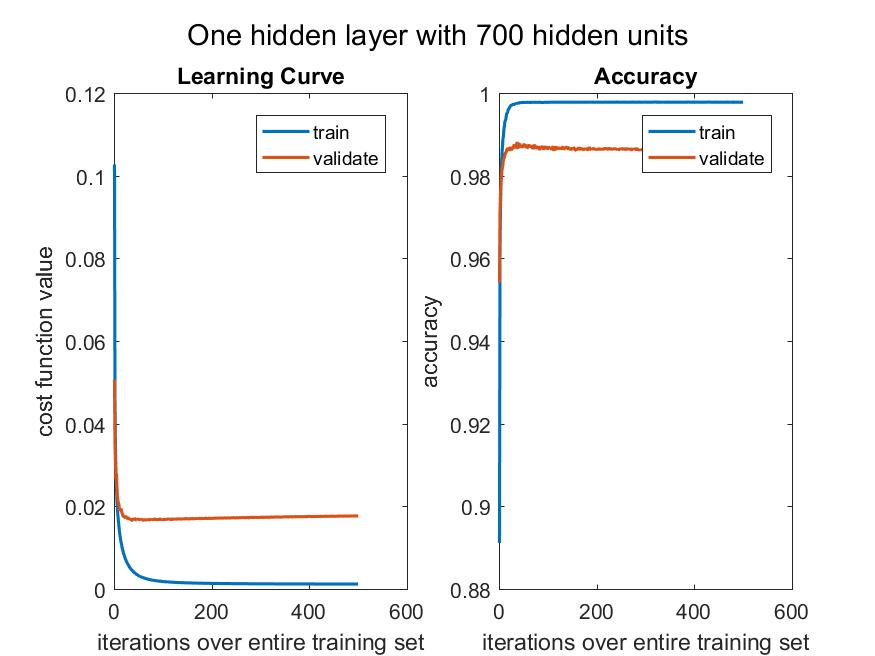
\includegraphics[width=3.5in]{LCAC700unitsPCA100eta.jpg}}
\caption{Left: learning curve of train set as well as validation set with 700 hidden units. Right: accuracy curve of train set as well as validation set with 700 hidden units.}
\label{1hidden700}
\end{figure}

\begin{figure}[h!]
\centerline{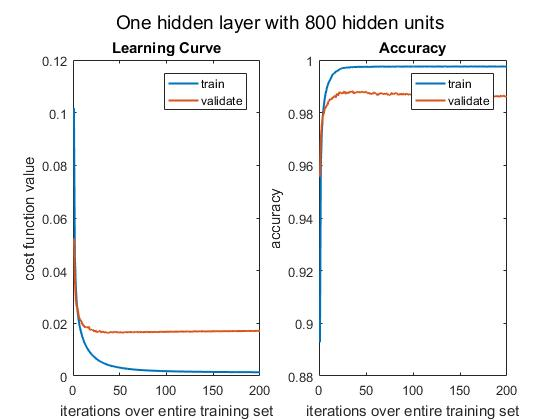
\includegraphics[width=3.5in]{LCAC800.jpg}}
\caption{Left: learning curve of train set as well as validation set with 800 hidden units. Right: accuracy curve of train set as well as validation set with 800 hidden units.}
\label{1hidden800}
\end{figure}

%\begin{figure}[htbp]
%\centerline{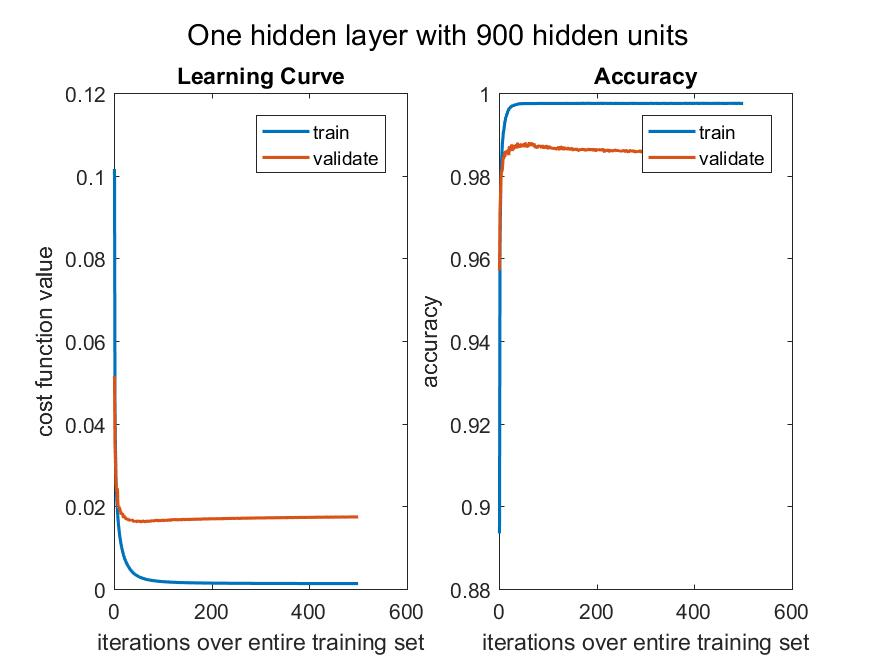
\includegraphics[width=3.5in]{LCAC900unitsPCA100eta.jpg}}
%\caption{Plot of fraction of total variance retained vs. number of eigenvalues}
%\label{1hidden900}
%\end{figure}

\begin{figure}[h!]
\centerline{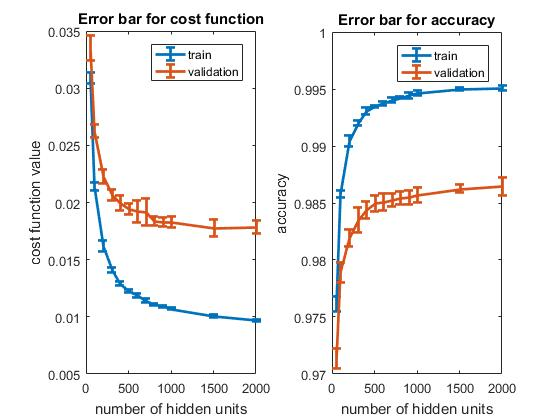
\includegraphics[width=3.5in]{errorbarAll.jpg}}
\caption{Plot of error bar with different number of hidden units}
\label{errorBar}
\end{figure}

\begin{table*}[h!]
\centering
\begin{tabular}{lccccccccccccc}
\hline
number of hidden units & 50 & 100 & 200 & 300 & 400 & 500 & 600 & 700 & 800 & 900 & 1000 & 1500 & 2000\\ \hline
average time for one epoch(s) & 2.7 & 6.5 & 11.9 & 14.9 & 17.3 & 18.5 & 19.7 & 21.78 & 22.6 & 25.19 & 26.9 & 32.7 & 46.9\\
average training cost & 0.0308 & 0.0214 & 0.0161 & 0.0141 &  0.0129 & 0.0123 & 0.0119 & 0.0114 & 0.0111 & 0.0109 & 0.0107 & 0.0101 & 0.0097\\
std.dev of training cost($\times 10^{-4}$) & 5.62 & 3.06 & 3.49 & 1.87&  2.15 & 1.36 & 1.57 & 1.30 & 0.788 & 0.978 & 0.885 & 0.985 & 0.865\\
average test accuracy(\%) &  97.08 &   97.86 &  98.28 & 98.46 & 98.49  & 98.56  & 98.56  & 98.61  & 98.60 &   98.62 & 98.66  & 98.70 & 98.69 \\
std.dev of test accuracy($\times 10^{-4}$) & 15 & 12 & 8.7280 & 8.1711 &  4.6774 & 3.8137 & 6.3805 & 4.7152 & 6.1833 & 5.0332 & 5.9442 & 3.4657 & 2.8284\\
\hline
\end{tabular}
\caption{Table of experiment results}
\label{tab: t1}
\end{table*}

As can be seen from the  learning curve, over-training is observed in every case given the iterations over the entire data set is large enough. Seen from the plot of error bar, as well as comparing the result in table \ref{tab: t1}, when the model is too complex, it would take too long to train and will improve the performance a little bit. So considering the training time-accuracy trade-off, for neural network with one hidden layer, the number of hidden units being 100 to 400 would be suitable and the single-hidden-layer neural network model with 100 hidden units will be experimented on later on.

\paragraph{Performance of the neural network with different step size}
Different step sizes are used and the learning curves are compared to select a suitable one. The learning curves are shown in figure \ref{LCSS}. It is not hard to find that the step size $\eta = 0.05$ is too large for the neural network to find the optimal solution with gradient descent, and the step size $\eta = 0.001$ is too small, lead to a slow convergence rate, which is not suitable since it takes too long the time to converge. Meanwhile, both $\eta = 0.01$ and $\eta = 0.005$ shows almost the same learning rate, with $\eta = 0.01$ slightly faster. 
\begin{figure}[h!]
\centerline{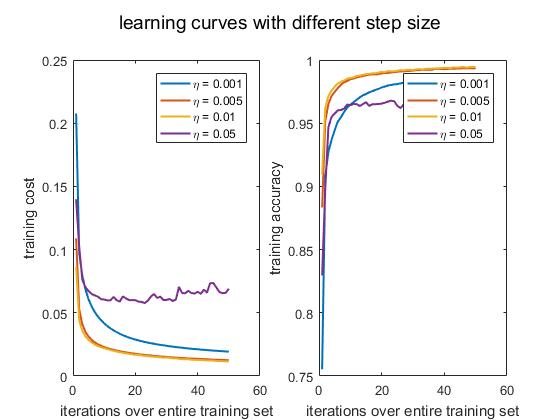
\includegraphics[width=3.5in]{noMOMENTUM.jpg}}
\caption{Learning curves with different step size.}
\label{LCSS}
\end{figure}

%The plots of weight tracks are shown in figure \ref{WT0005} and \ref{WT001}.
%\begin{figure}[h!]
%\centerline{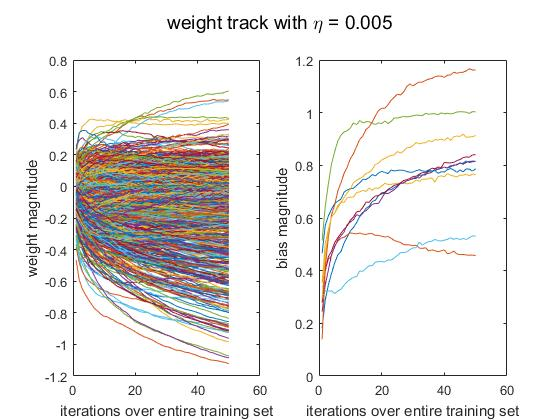
\includegraphics[width=3.5in]{WT0005.jpg}}
%\caption{Weight track with step size $\eta = 0.005$.}
%\label{WT0005}
%\end{figure}

%\begin{figure}[h!]
%\centerline{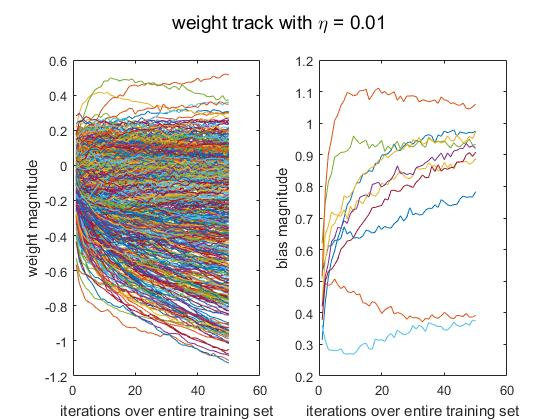
\includegraphics[width=3.5in]{WT001.jpg}}
%\caption{Weight track with step size $\eta = 0.01$.}
%\label{WT001}
%\end{figure}

\paragraph{Performance of the neural network with different dimension retained}
As mentioned before, keeping dimension of 100 is a good starting point, experiments are also done to discuss this problem. As shown in table \ref{tab: t2} and figure \ref{errorBarPCA}, are the comparison of performance of the model with different dimensions being retained of the original dataset. The step size is set to be 0.01. The same experiment is run 10 times to compare the average and standard deviation of the accuracy to compare the performance.\\
\begin{table*}[h!]
\centering
\begin{tabular}{lccccc}
\hline
number of dimension retained & 50 & 100 & 200 & 400 & 781\\
\hline
average time for one epoch(s) &  2.4 &  2.9 & 6.3 & 9.5 & 13.5\\
average training accuracy(\% )  & 98.10 &  98.59 & 98.86 & 98.98 & 99.02\\
std.dev of training accuracy($\times 10^{-4}$) & 4.2619 & 4.0378 & 3.5405 & 2.8697 & 3.9001\\
average test accuracy(\% ) & 97.66 & 97.65 & 97.85 & 97.84 & 97.87\\
std.dev of test accuracy($\times 10^{-4}$) & 11 & 13 & 8.5797 & 9.1196 & 12\\
\hline
\end{tabular}
\caption{Table of experiment results with different dimensionality retained by PCA}
\label{tab: t2}
\end{table*}

\begin{figure}[h!]
\centerline{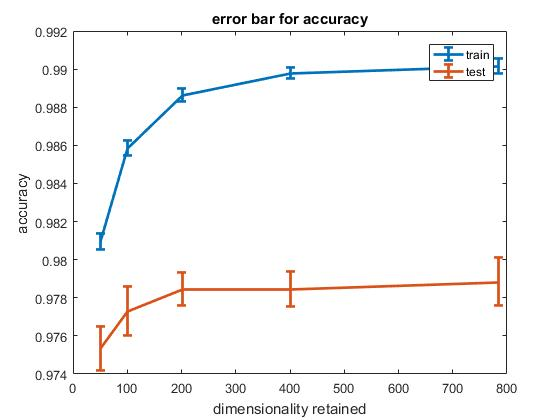
\includegraphics[width=3.5in]{PCAerrorBar.jpg}}
\caption{Plot of error bar with different number of dimensionality retained.}
\label{errorBarPCA}
\end{figure}

\paragraph{Performance of the neural network with momentum term} 
The comparison of the whether to include the momentum term is done by comparing the output weight (bias) of the network. The the weight tracks of then network without momentum term is shown in figure \ref{WTno}, the weight tracks of the network with momentum term is shown in figure \ref{WTM}.
%\begin{figure}[htbp]
%\centerline{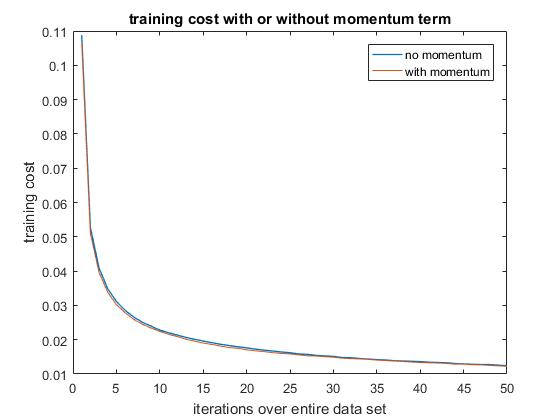
\includegraphics[width=3.5in]{LCcomM.jpg}}
%\caption{Weight track without momentum term step size $\eta = 0.05$.}
%\label{LCcomM}
%\end{figure}

\begin{figure}[h!]
\centerline{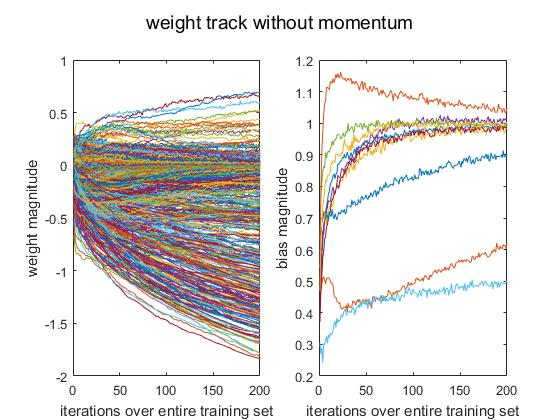
\includegraphics[width=3.5in]{noMeta0010.jpg}}
\caption{Weight track without momentum term step size $\eta = 0.05$. Left: output weight. Right: output bias.}
\label{WTno}
\end{figure}

\begin{figure}[h!]
\centerline{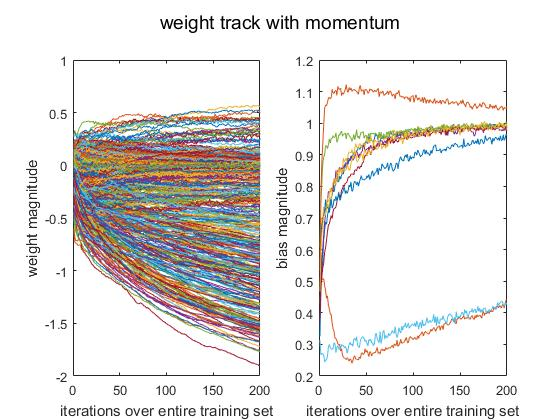
\includegraphics[width=3.5in]{Meta0010.jpg}}
\caption{Weight track without momentum term step size $\eta = 0.05$. Left: output weight. Right: output bias.}
\label{WTM}
\end{figure}

\paragraph{Performance of the neural network with dropout}
The plot of test accuracy versus  iterations over entire training set is shown below in figure \ref{dO}.
\begin{figure}[h!]
\centerline{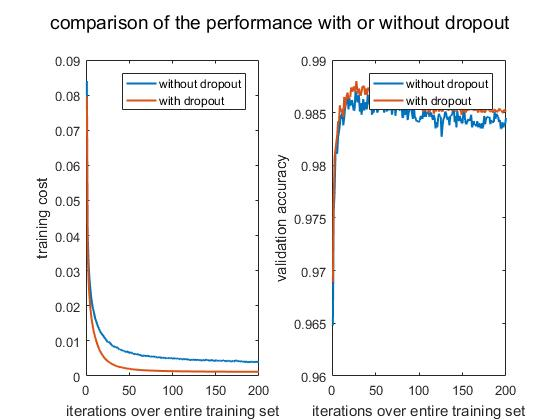
\includegraphics[width=3.5in]{dropoutPlot.jpg}}
\caption{Comparison of the performance of the same neural network, with or without dropout.}
\label{dO}
\end{figure}


\paragraph{Confusion matrix on the test set}
The final model is chosen to the one trained by one hidden layer neural network, with 100 hidden units, and the data set is project to a subspace of dimensionality 100, the test accuracy on the test is 97.86\%, the confusion matrix is shown below in figure \ref{confu}:
\begin{figure}[h!]
\centerline{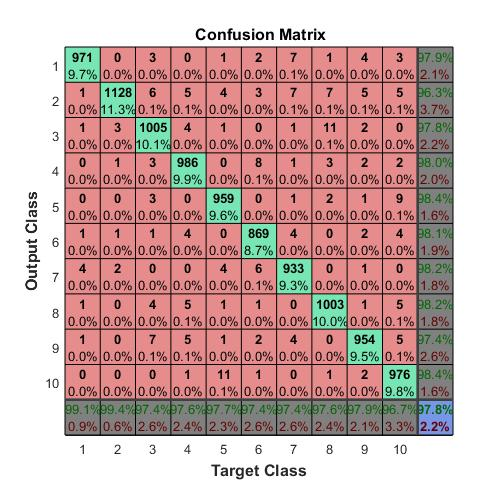
\includegraphics[width=3.5in]{confu.jpg}}
\caption{Confusion matrix for the final model test no the test data set, where ``class 1" represent for number ``0", and so forth.}
\label{confu}
\end{figure}


\section{Discussion}
Given the problem with many parameters influenced by each other, especially more than 3 parameters as this case, the visualization of all parameters working together would be hard. And at the same time, for every training procedure, the initialization is random. And the learning procedure of neural networks depend on initialization a lot. Taking ReLU activation function as example, as shown and discussed before, ReLU function is highly sensitive to the step size, resulting from its sensitivity to the input value, i.e. a large input value would ``kill" the network. It is true for other activation functions. Considering the training procedure for neural networks is initialization dependent, it is necessary to repeat the training procedure with different initialization several times, and compare the result as well as the variance of the result.

Learn from the Curse of Dimensionality, the dimensionality reduction is always important and necessary in machine learning. As shown in figure \ref{PCA}, keeping dimension of the data set to be 100 would keep 90\% of the variance of the original data set, which is higher than generally using 85\%. Though it is always necessary to test the performance on the data set we are dealing with - the dimensionality to be kept is higher depend on the problem and the desired performance, so experiments are necessary. And as shown in table \ref{tab: t2}, with the number of hidden units set to be 100, the performance of the neural network is compared with different dimensionality of data being retained. As we can see, the accuracy of the training set kept increasing with the increasing of number of dimension retained, the accuracy of the mode when test on the test set actually decreases. While if the number of dimension retained is too small, i.e. 50 in the experiment described above, the retained variance is not enough to represent the original data set. Thus, for this problem, projecting the original data set to the space with dimensionality of 100 to 200 is a good choice.

After repeating the experiment on models with different number of hidden units 10 times, and compare the result, as shown in table \ref{tab: t1} and figure \ref{errorBar}, it is obvious that with more hidden units, i.e. more complex model, the performance would be better for training set as well as validation set, but actually the performance of validation set starting to stop changing. Also as is shown in the table \ref{tab: t1}, more complex model will not improve the performance significantly better, while with a cost of longer training time, which means less efficiency, and with a higher probability of over training. So a choosing a much simpler model would be wise, i.e. choosing the number of hidden units to be 100 to 400. 

When it comes to the matter of the learning rate $\eta$, it is actually depending on the model and other parameters. If the model is set to be one hidden layer network with 700 hidden units, and the dimensionality of the data is set to be 100, then it is obvious from figure \ref{LCSS}, that for this model, step size $\eta = 0.05$ is too large for the network to be able to converge. As a matter of fact, the ReLU activation function is highly sensitive to the step size, resulting from it is sensitive to the input value, for example, a large gradient flowing through a ReLU neuron could cause the weights to update in such a way that the neuron will never activate on a data point again. Especially when setting the learning rate being too large\cite{b5}. Thus it is always necessary to set the learning rate to be a small one when using ReLU function to be the activation function. And also, it is obvious in this problem that using step sizes either $\eta = 0.005$ or $\eta = 0.01$ will not affect the learning procedure much.

When considering the momentum term, as shown in figures \ref{WTno} and \ref{WTM}, which is much obvious as is shown in the bias track, two experiments start at the same initial values of weights and biases, the learning procedure with momentum term updates the weights/biases differently from the one without momentum term, i.e., when the updating step is toward a wrong direction, it corrects the direction by updating with a smaller step size to the wrong direction. What is more, the parameter $\alpha$ for the momentum is another hyper-parameter which can be further discussed regarding its performance.

When looking at the final confusion matrix, though the overall performance of the network gained a small error rate of $2.14\%$, there is still some error observed, i.e. there are still off-diagonal entries populated. When looking at the confusion matrix closely, it is not hard to observe that the there is some probability for the number ``0" (target class 1 as shown in the confusion matrix) to be misclassified as ``6" (output class 7), and there is also some probability for the number ``6" to be misclassified as ``0", both of the situation make sense since when looking at the images of these numbers, some handwritten numbers are not so clear, which leads to the misclassification. The similar situation happen with a higher probability when the number ``4"(target class 5) being misclassified as number ``9"(output class 10). This kind of situation occurs due to different hand written behavior recorded in this MNIST data set.

	
\section{Conclusions}  
In this paper the performance of artificial neural network with one hidden unit was examined with regard to several aspects: the dimensionality of the input data, the architecture of the model (i.e. the number of hidden units), the learning rate, the inclusion of the momentum term.

Given a problem with more than three parameters working together and influence with each other, it is hard to decide one set of the best ones together. Thus it is necessary to repeat the whole training procedure several times to compare the final results, as done in this report.

For this specific problem, if only one hidden layer is used, the number of units being 100 to 400 should be enough for the network to have a good performance. For the activation function, there is no ``best one" but a suitable one, but with different activation function, the initialization step as well as the learning rate should be adjusted accordingly. 

Only one hidden layer neural network is discussed in this paper, including hidden layers may improve the accuracy, and need to be experimented on as future work. And what is more, mini batch can also be used in network training and the batch size can be discussed with regard to the network performance as future work.


\begin{thebibliography}{00}
\bibitem{b1} https://en.wikipedia.org/wiki/MNIST\_database
\bibitem{b2} Principe, Jose C., Euliano Neil R. and Lefebvre W. Curt. ``Neural and Adaptive Systems: Fundamentals through Simulations." (1991): chapter 3.
\bibitem{b3} Elements of Machine Intelligence lecture notes.
\bibitem{b4} Srivastava, Nitish, Hinton., Hinton, Geoffrey., Krizhevsky, Alex. etc. `` Dropout: A Simple Way to Prevent Neural Networks from Overfitting." Journal of Machine Learning Research 15 (2014) 1929-1958.
\bibitem{b5} http://cs231n.github.io/neural-networks-1/
\bibitem{b6} http://davidstutz.de/wordpress/wp-content/uploads/2014/03/seminar.pdf
\end{thebibliography}

\emph{I confirm that this assignment is my own work, is not copied from any other's work (published or unblished), and has not been previously submitted for assessment either at University of Florida or elsewhere.}
	\begin{figure}[htbp]
	\centerline{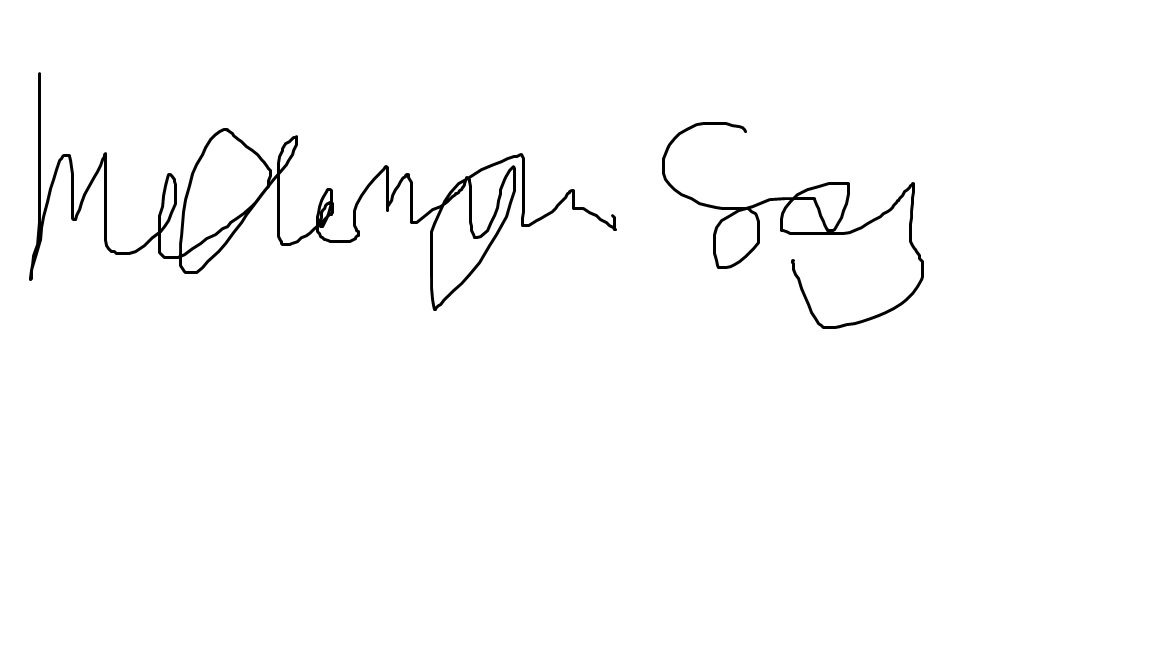
\includegraphics[width=3.4in]{sig.jpg}}
	\end{figure}

\end{document}
